\documentclass[UTF8, a4paper]{ctexart}
\usepackage{titlesec}
\usepackage{graphicx}
\usepackage{amsmath}
\usepackage{tabularx}
\usepackage[top=2cm, bottom=2cm, left=2cm, right=2cm]{geometry}
% 设置节标题左对齐
\titleformat{\section}[block]{\normalfont\Large\bfseries}{\thesection}{1em}{}

\title{计算机模拟物理大作业}
\author{夏泽宇}
\begin{document}
\maketitle
\section{悬挂系统的数学模型}

\begin{figure}[h]
    \centering
    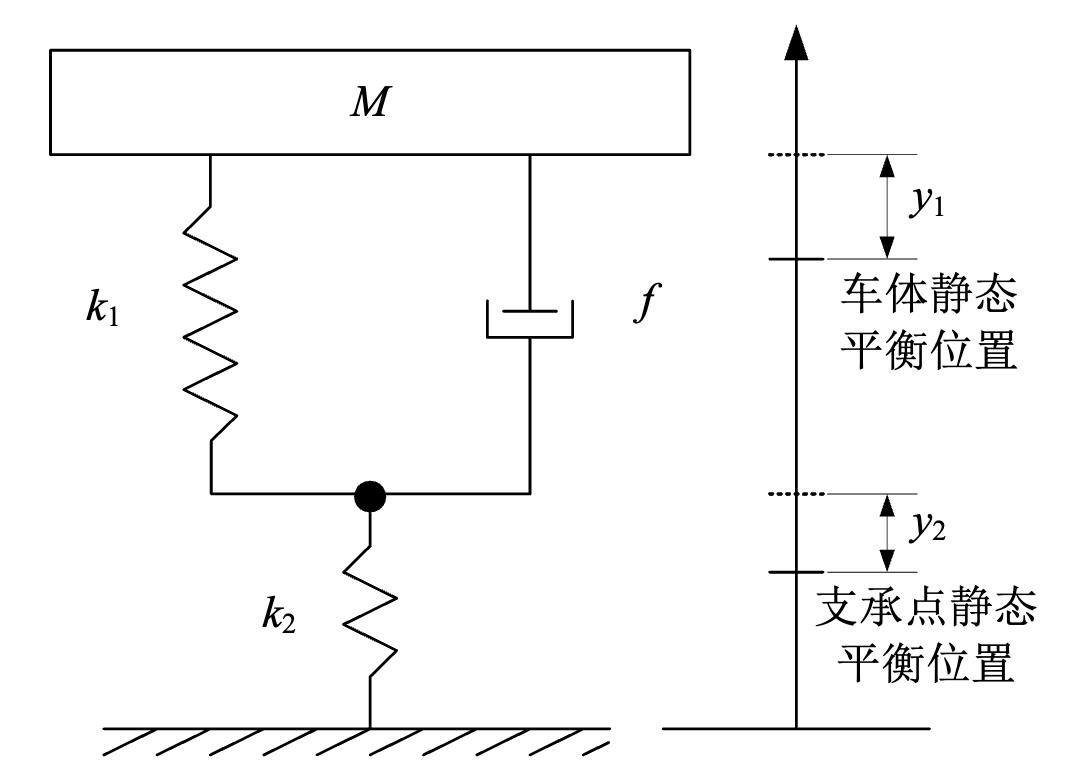
\includegraphics[width=0.5\textwidth]{../fig/schematic.jpeg}
    \caption{示意图}
    \label{fig:schematic}
\end{figure}
如上图所示,设车体质量的1/4为$M$,轮胎质量为$m$,$k_1$为车弹簧弹性系数,
$k_2$为轮胎弹性系数。减震阻尼不承重,仅提供阻尼$f$。

考虑车体的运动方程,设车体相对平衡位置的位移为$y_1$,轮胎(支承点)相对平衡位置的位移为$y_2$,则有:
\begin{equation}
    \begin{aligned}
        M\ddot{y_1} &= -f(\dot{y_1}-\dot{y_2}) - k_1(y_1 - y_2)\\
        m\ddot{y_2} &= f(\dot{y_1}-\dot{y_2}) + k_1(y_1 - y_2) - k_2y_2
    \end{aligned}
    \label{eq:kinematics}
\end{equation}

将式(\ref{eq:kinematics})改写为矩阵形式,有:
\[
\begin{bmatrix}
    M & 0 \\
    0 & m
\end{bmatrix}
\begin{bmatrix}
    \ddot{y_1} \\
    \ddot{y_2}
\end{bmatrix}
+
\begin{bmatrix}
    f & -f \\
    -f & f
\end{bmatrix}
\begin{bmatrix}
    \dot{y_1} \\
    \dot{y_2}
\end{bmatrix}
+
\begin{bmatrix}
    k_1 & -k_1 \\
    -k_1 & k_1 + k_2
\end{bmatrix}
\begin{bmatrix}
    y_1 \\
    y_2
\end{bmatrix}
=
\begin{bmatrix}
    0 \\
    0
\end{bmatrix}
\]

\[
A=\begin{bmatrix}
    M & 0 \\
    0 & m
\end{bmatrix},B=\begin{bmatrix}
    f & -f \\
    -f & f
\end{bmatrix},C=\begin{bmatrix}
    k_1 & -k_1 \\
    -k_1 & k_1 + k_2
\end{bmatrix}
\]

\begin{equation}
    A\ddot{y} + B\dot{y} + Cy = 0
    \label{eq:matrix}
\end{equation}

考虑上述二阶常微分方程组的特征方程,其特征矩阵为:
\[
\begin{bmatrix}
    0 & I \\
    -A^{-1}C & -A^{-1}B
\end{bmatrix}
\]

代入具体值即可通过计算得到特征值,其虚部表征了系统的特征频率。

\section{悬挂系统的数值模拟}

\subsection{特征频率}
通过查阅资料,得到了悬挂系统的参数,如下表所示:
\begin{table}[h]
    \centering
    \begin{tabularx}{\textwidth}{|X|X|X|X|X|X|}
        \hline
        参数 & $M$ & $m$ & $k_1$ & $k_2$ & $f$ \\
        \hline
        数值 & 500kg & 50kg & 20kN/m & 200kN/m & 200N$\cdot$s/m \\
        \hline
    \end{tabularx}
    \caption{悬挂系统参数}
    \label{tab:parameters}
\end{table}

在此参数下,通过计算得到特征频率为:10.5550Hz、0.9591Hz。

计算过程见于code文件夹下的frequency.m代码。

\subsection{阶跃响应}
考虑在$t=0$时刻,轮胎受到一个冲量,使轮胎有向上的位移和速度,无妨设为即$y_2(0)=1$,$\dot{y_2}(0)=1$。
通过模拟车辆的运动,得到$y_1$和$y_2$的变化情况,如下图所示:
\begin{figure}[h]
    \centering
    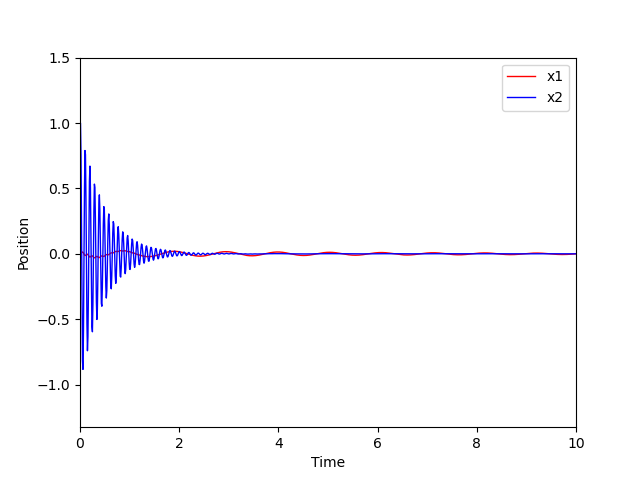
\includegraphics[width=0.8\textwidth]{../fig/step_response.png}
    \caption{阶跃响应}
    \label{fig:step_response}
\end{figure}

在此冲击下,0时刻轮胎相较平衡位置有一个较大的位移和速度,但由于弹簧和阻尼器的作用,振幅很快衰减。
一部分能量同时传播到车身上,使车身发生振动。整个过程中,轮胎的位移和速度有一个较大的变化,其振幅为0.901m;
但是车体的位移和速度变化较小,其振幅为0.0223m说明悬挂系统的减震效果较好。

\clearpage
\subsection{正弦响应}
考虑从$t=0$时起,轮胎受到一个周期性的正弦信号,$f(t)=1000sin(2\pi f t+\frac{\pi}{2})$,同上面一样,设初始条件为$y_2(0)=1$,$\dot{y_2}(0)=1$。
取正弦信号的频率为特征频率10.5550Hz,通过模拟车辆的运动,得到$y_1$和$y_2$的变化情况,如下图所示:

\begin{figure}[h]
    \centering
    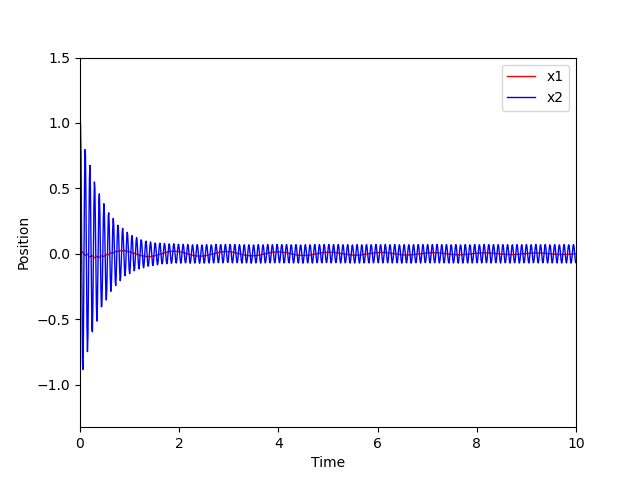
\includegraphics[width=0.65\textwidth]{../fig/sine_response.png}
    \caption{正弦响应}
    \label{fig:sin_response}
\end{figure}

可以看到,在此特征频率下,轮胎的振幅较大,为0.0717m,而车体的振幅依然很小,为0.0118m。
特征频率是同等振幅下引起车身振幅最大的振动频率,在此频率下的车身振幅完全是可接受的,这证实了减震系统的有效性。

\subsection{幅频特性}
对于频率变化的正弦激励信号$f(t)=1000sin(2\pi f t+\frac{\pi}{2})$, $f$从0Hz到15Hz变化。
通过模拟车辆的运动,得到$y_1$和$y_2$对应振幅的变化情况,如下图所示:

\begin{figure}[h]
    \centering
    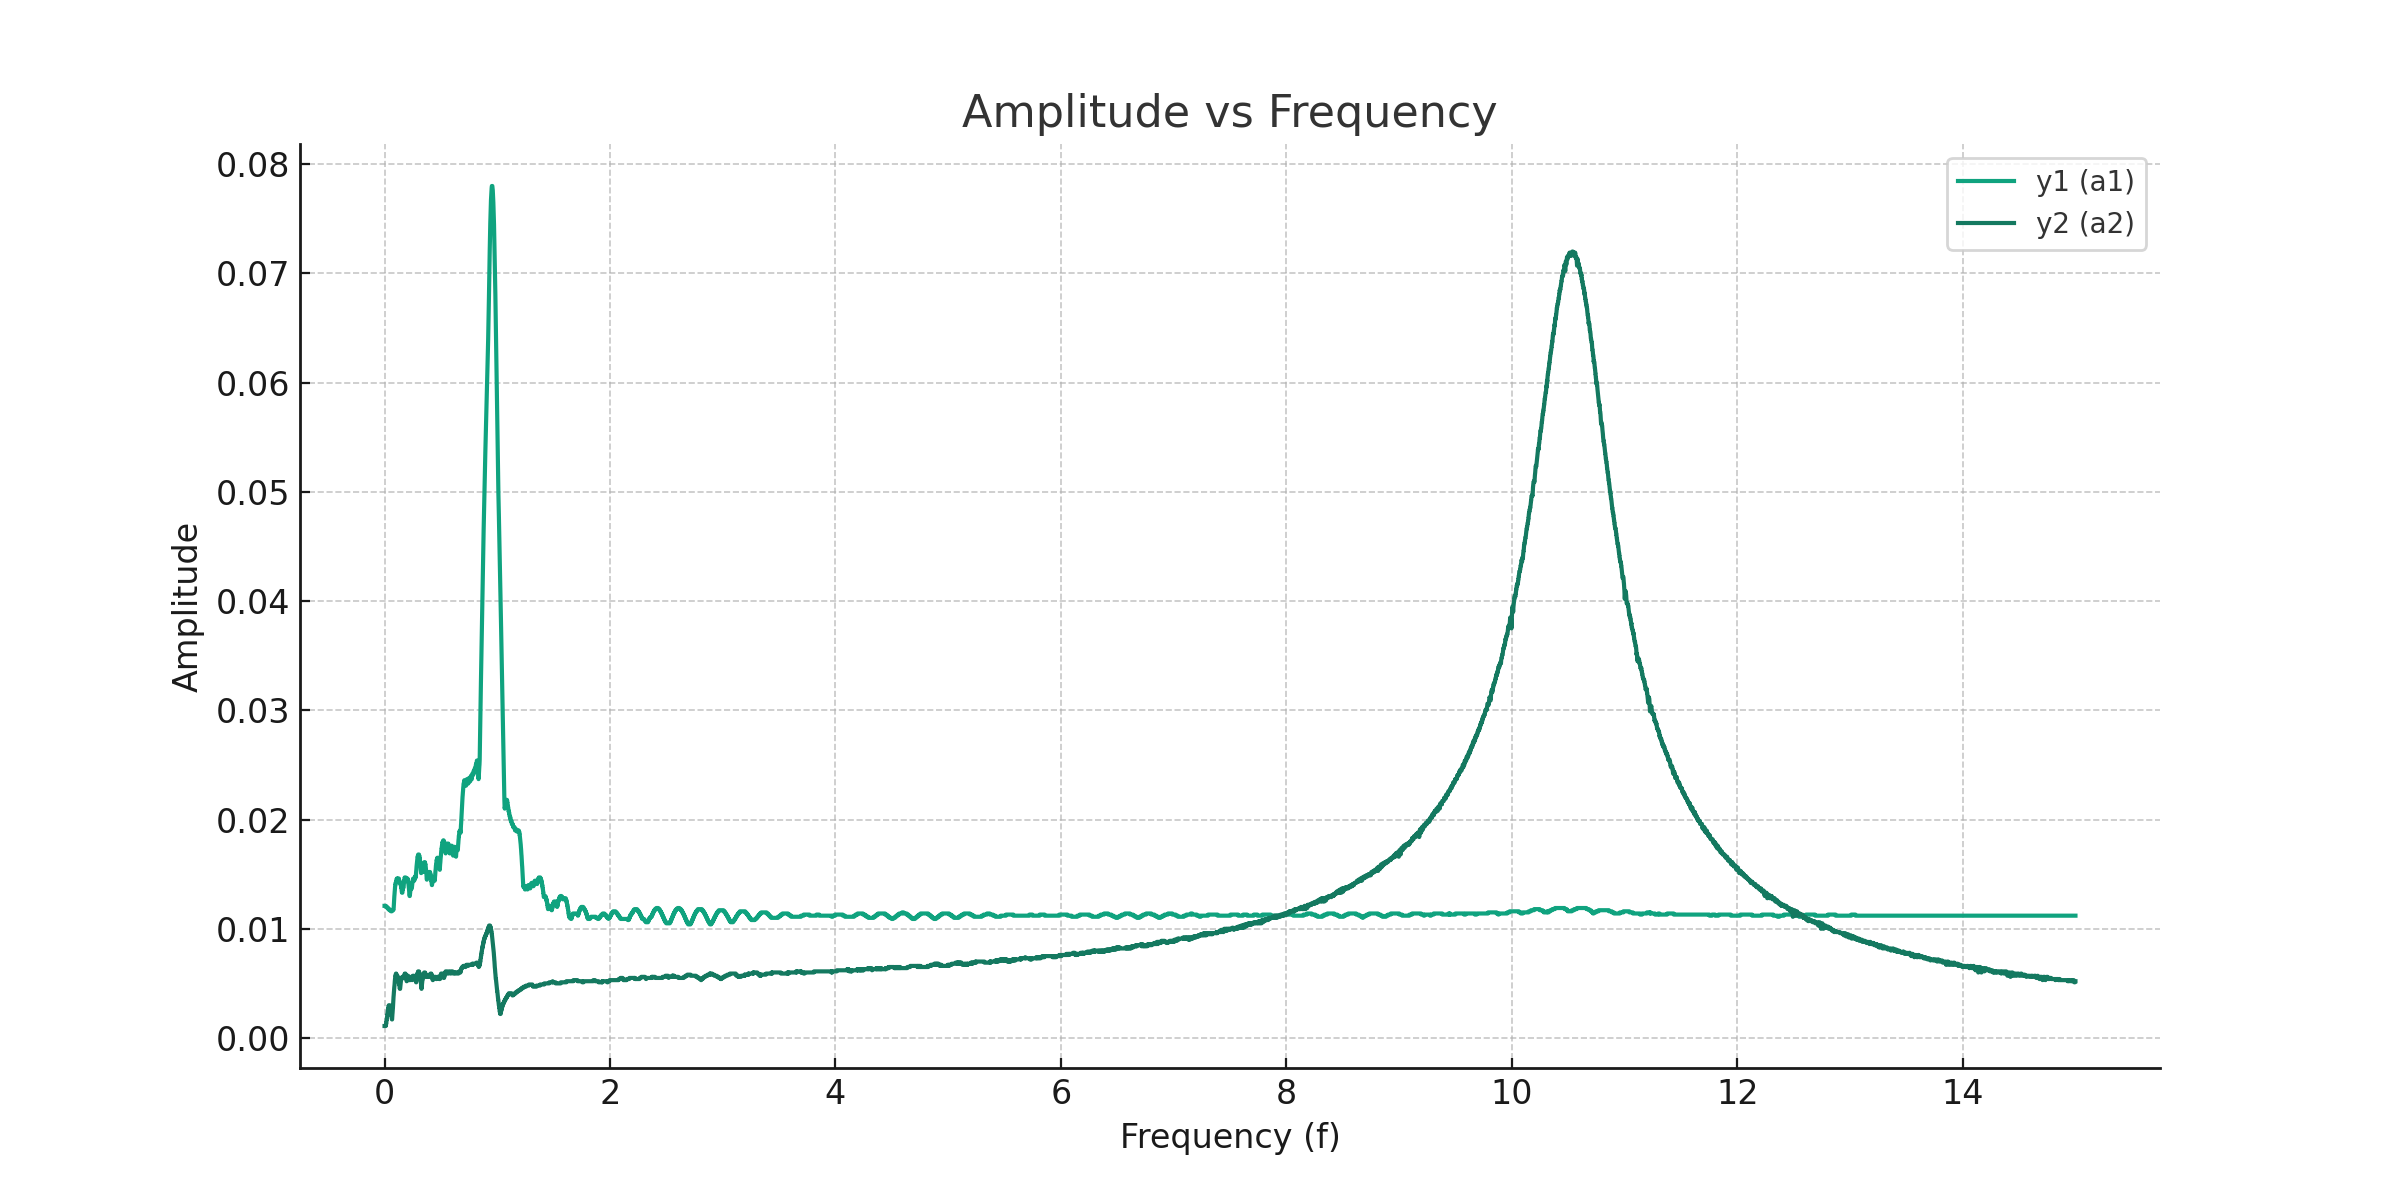
\includegraphics[width=0.7\textwidth]{../fig/amplitude_vs_frequency.png}
    \caption{幅频特性曲线}
    \label{fig:amplitude_frequency}
\end{figure}

从图中可以看出,幅频特性曲线的2个极大值就是前面计算得到的特征频率,这印证了计算过程的正确性。

\section{总结}
通过对悬挂系统的数学模型的建立,可以得到悬挂系统的特征频率;
通过对悬挂系统的数值模拟,可以得到悬挂系统的阶跃响应、正弦响应和幅频特性曲线。
在选定参数下,对悬挂系统在不同激励下的响应进行了分析,并测得了幅频特性曲线。多重实验结果表明了悬挂系统的有效性。

\end{document}

